\begin{figure}[H]
    \begin{subfigure}{0.5\textwidth}
        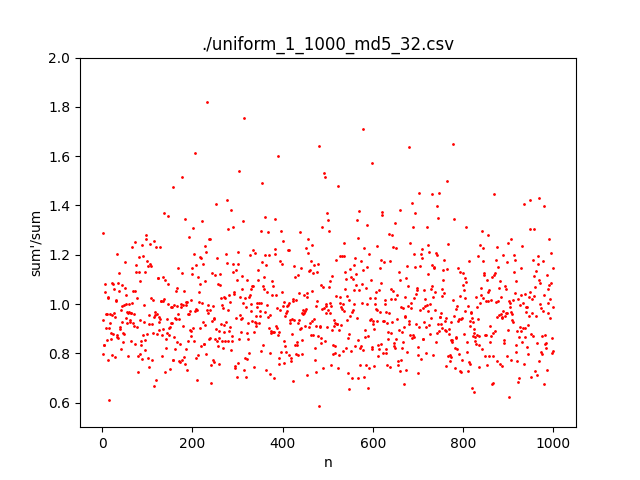
\includegraphics[width=1.0\linewidth, height=5cm]{uniform_1_1000/uniform_1_1000_md5_32.png}
        \caption{$m = 32$}
        \label{fig:subim1}
    \end{subfigure}
    \begin{subfigure}{0.5\textwidth}
        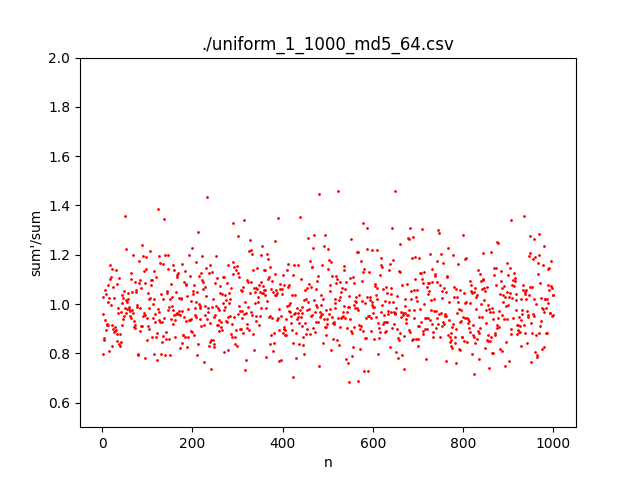
\includegraphics[width=1.0\linewidth, height=5cm]{uniform_1_1000/uniform_1_1000_md5_64.png}
        \caption{$m = 64$}
        \label{fig:subim1}
    \end{subfigure}
    \begin{subfigure}{0.5\textwidth}
        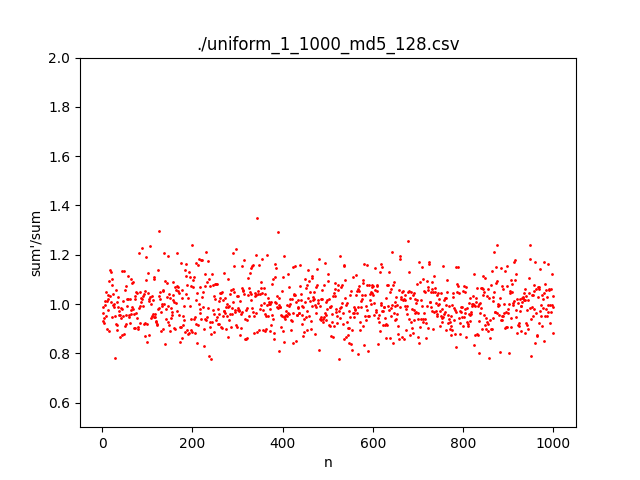
\includegraphics[width=1.0\linewidth, height=5cm]{uniform_1_1000/uniform_1_1000_md5_128.png}
        \caption{$m = 128$}
        \label{fig:subim2}
    \end{subfigure}
    \begin{subfigure}{0.5\textwidth}
        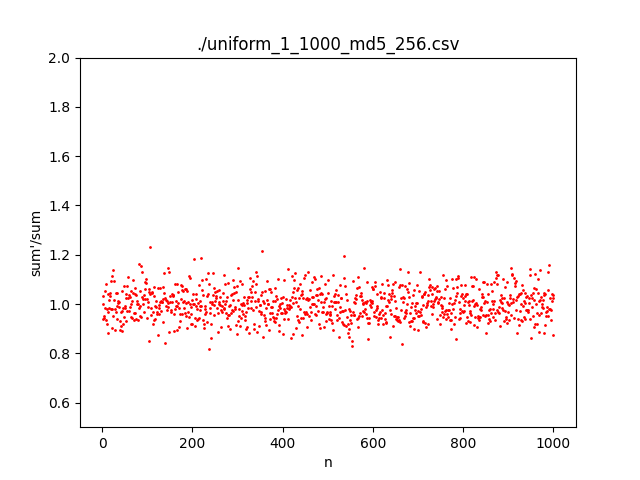
\includegraphics[width=1.0\linewidth, height=5cm]{uniform_1_1000/uniform_1_1000_md5_256.png}
        \caption{$m = 256$}
        \label{fig:subim2}
    \end{subfigure}

    \caption{Wykresy przedstawiają wyniki algorytmu dla różnej ilości rejestrów gdy wartości cech pochodzą z rozkładu jednostajnego na przedziale $[1, 1000]$. Wykorzystany algorytm: \texttt{md5}.}
    \label{fig:uniform_md5}
\end{figure}

\begin{figure}[H]
    \begin{subfigure}{0.5\textwidth}
        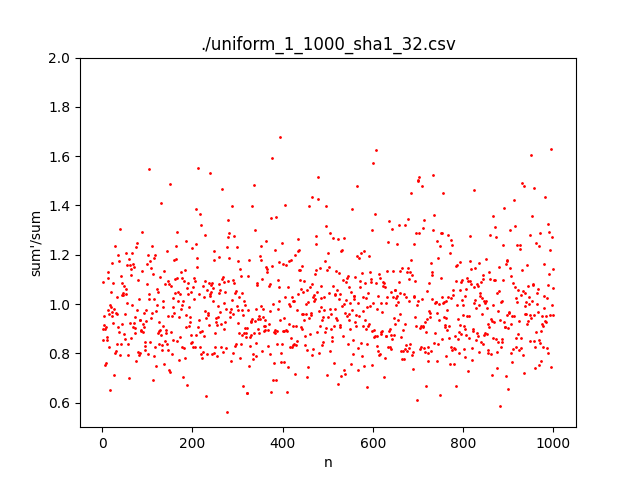
\includegraphics[width=1.0\linewidth, height=5cm]{uniform_1_1000/uniform_1_1000_sha1_32.png}
        \caption{$m = 32$}
        \label{fig:subim1}
    \end{subfigure}
    \begin{subfigure}{0.5\textwidth}
        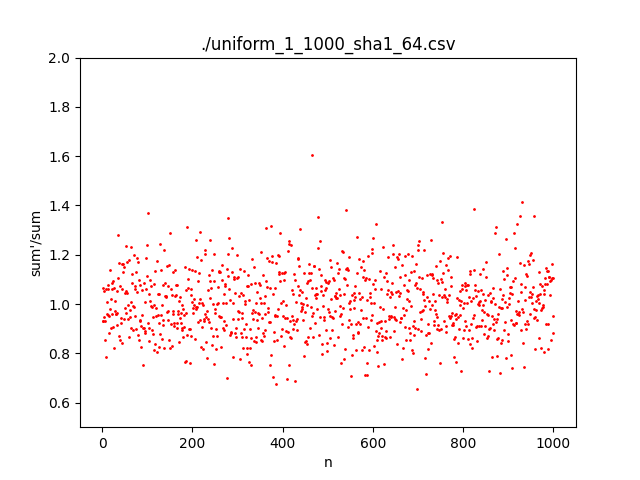
\includegraphics[width=1.0\linewidth, height=5cm]{uniform_1_1000/uniform_1_1000_sha1_64.png}
        \caption{$m = 64$}
        \label{fig:subim1}
    \end{subfigure}
    \begin{subfigure}{0.5\textwidth}
        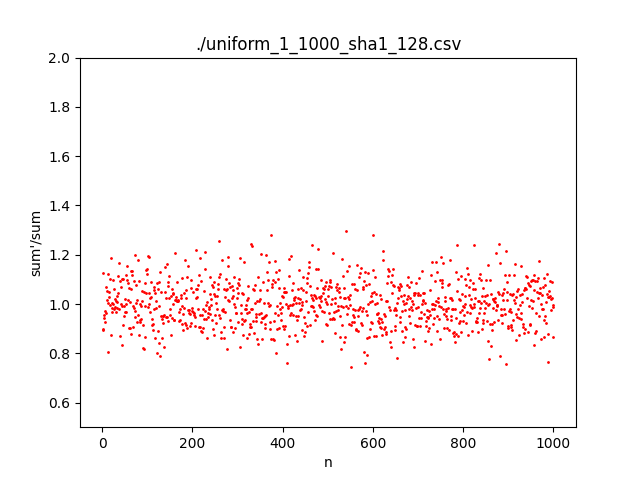
\includegraphics[width=1.0\linewidth, height=5cm]{uniform_1_1000/uniform_1_1000_sha1_128.png}
        \caption{$m = 128$}
        \label{fig:subim2}
    \end{subfigure}
    \begin{subfigure}{0.5\textwidth}
        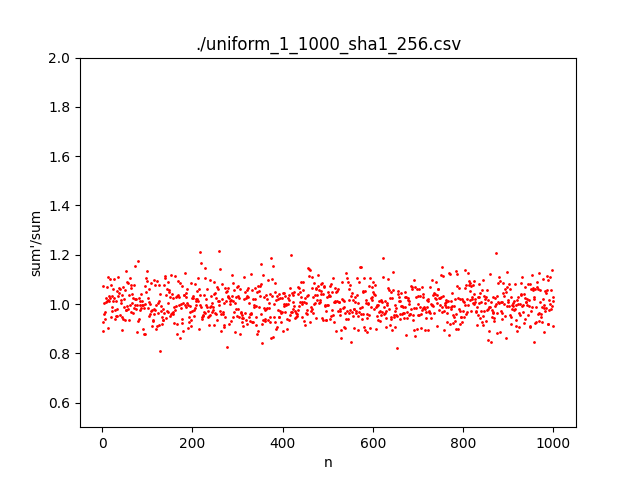
\includegraphics[width=1.0\linewidth, height=5cm]{uniform_1_1000/uniform_1_1000_sha1_256.png}
        \caption{$m = 256$}
        \label{fig:subim2}
    \end{subfigure}

    \caption{Wykresy przedstawiają wyniki algorytmu dla różnej ilości rejestrów gdy wartości cech pochodzą z rozkładu jednostajnego na przedziale $[1, 1000]$. Wykorzystany algorytm: \texttt{sha1}.}
    \label{fig:uniform_sha1}
\end{figure}

\begin{figure}[H]
    \begin{subfigure}{0.5\textwidth}
        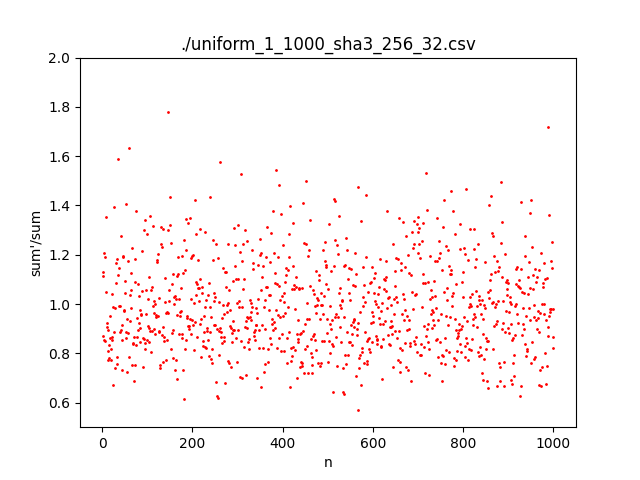
\includegraphics[width=1.0\linewidth, height=5cm]{uniform_1_1000/uniform_1_1000_sha3_256_32.png}
        \caption{$m = 32$}
        \label{fig:subim1}
    \end{subfigure}
    \begin{subfigure}{0.5\textwidth}
        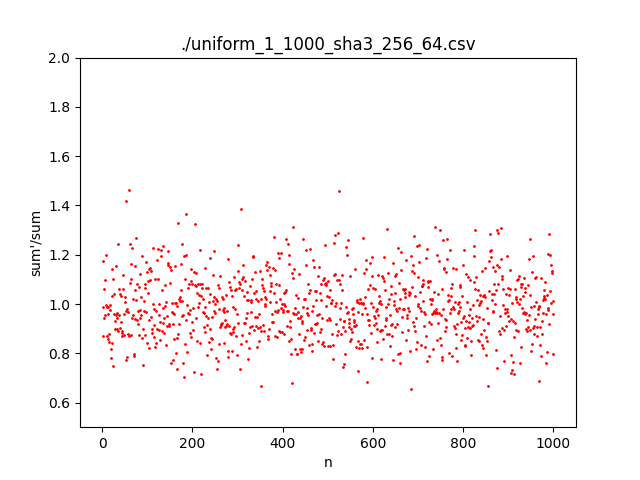
\includegraphics[width=1.0\linewidth, height=5cm]{uniform_1_1000/uniform_1_1000_sha3_256_64.png}
        \caption{$m = 64$}
        \label{fig:subim1}
    \end{subfigure}
    \begin{subfigure}{0.5\textwidth}
        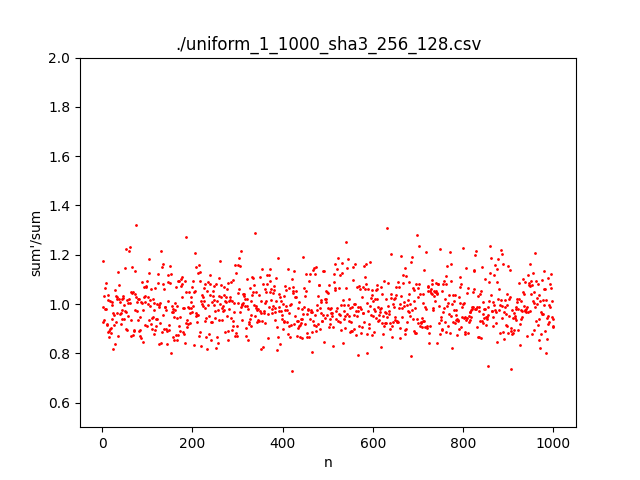
\includegraphics[width=1.0\linewidth, height=5cm]{uniform_1_1000/uniform_1_1000_sha3_256_128.png}
        \caption{$m = 128$}
        \label{fig:subim2}
    \end{subfigure}
    \begin{subfigure}{0.5\textwidth}
        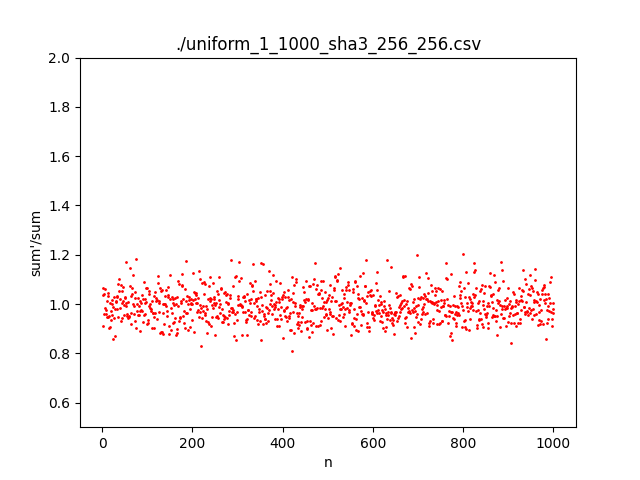
\includegraphics[width=1.0\linewidth, height=5cm]{uniform_1_1000/uniform_1_1000_sha3_256_256.png}
        \caption{$m = 256$}
        \label{fig:subim2}
    \end{subfigure}

    \caption{Wykresy przedstawiają wyniki algorytmu dla różnej ilości rejestrów gdy wartości cech pochodzą z rozkładu jednostajnego na przedziale $[1, 1000]$. Wykorzystany algorytm: \texttt{sha3}.}
    \label{fig:uniform_sha3_256}
\end{figure}
